% Fig1 — where a corrupted attribution enters an agentic SOC, and what it costs.
%
% Conceptual, so it is drawn rather than plotted, but the source lives in the repo like
% every other float. The point of the figure is the asymmetry: the prediction path is
% monitored and the explanation path is not, and the consumer at the end of the
% explanation path is now a machine that acts in seconds.
%
%   pdflatex -output-directory=figures/out figures/src/fig1_threat_schematic.tex
%
% Colours are the Okabe-Ito steps used by figures/src/style.py, checked with
% figures/src/check_palette.py.

\documentclass[border=2pt]{standalone}
\usepackage{tikz}
\usepackage{xcolor}
\usetikzlibrary{arrows.meta, positioning, fit, backgrounds, calc}

\definecolor{okblue}{HTML}{0072B2}
\definecolor{okorange}{HTML}{D55E00}
\definecolor{okgreen}{HTML}{009E73}
\definecolor{inkmuted}{HTML}{595959}

\begin{document}
% Fig1 body — \input this straight into the paper, whose preamble already loads tikz
% with arrows.meta, positioning, fit, backgrounds and calc. The standalone wrapper
% fig1_threat_schematic.tex exists only for previewing the figure on its own.
% Colour definitions live in the wrapper; the paper defines them once in its preamble.

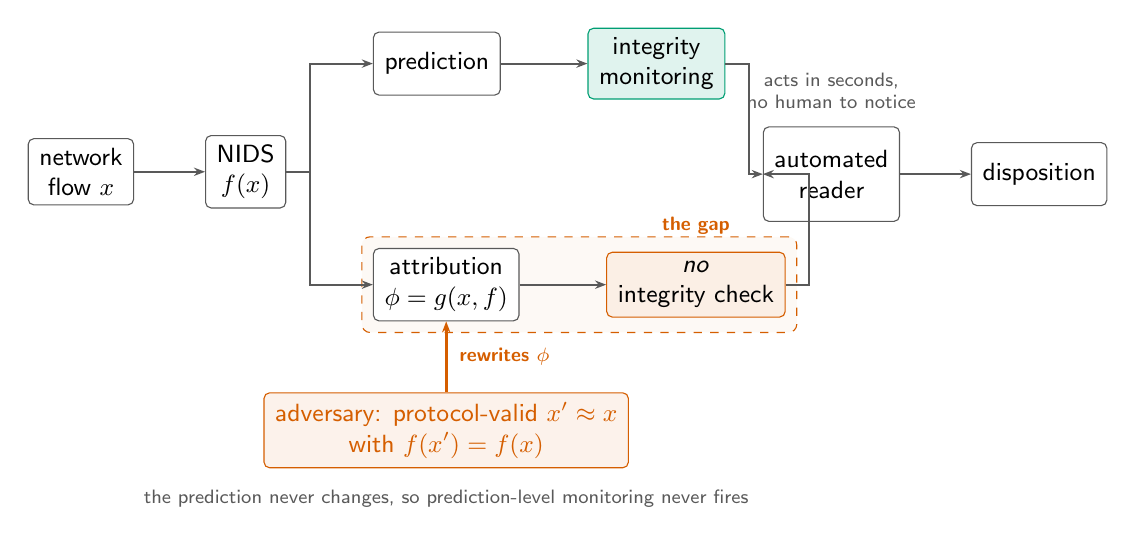
\begin{tikzpicture}[
  font=\sffamily\small,
  box/.style   = {draw=inkmuted, rounded corners=2pt, minimum height=8mm,
                  inner xsep=4pt, align=center, fill=white},
  flow/.style  = {-{Stealth[length=4pt]}, draw=inkmuted, line width=0.7pt},
  bad/.style   = {-{Stealth[length=4pt]}, draw=okorange, line width=1.1pt},
  lbl/.style   = {font=\sffamily\scriptsize, text=inkmuted, align=center},
  badlbl/.style= {font=\sffamily\scriptsize\bfseries, text=okorange, align=center},
]

% ---- the pipeline
\node[box] (flowin)   {network\\flow $x$};
\node[box, right=9mm of flowin]  (nids)   {NIDS\\$f(x)$};
\node[box, above right=5mm and 11mm of nids] (pred)  {prediction};
\node[box, below right=5mm and 11mm of nids] (expl)  {attribution\\$\phi = g(x,f)$};
\node[box, right=11mm of pred, fill=okgreen!12, draw=okgreen] (mon) {integrity\\monitoring};
\node[box, right=11mm of expl, fill=okorange!10, draw=okorange] (none) {\emph{no}\\integrity check};
% "automated reader", never "agent": the paper's one term for the consumer
% (Main.tex \reader). "disposition" not "containment
% action" — the experiment measures a committed choice, not an executed action.
\node[box, right=11mm of $(mon)!0.5!(none)$, minimum height=12mm] (agent)
      {automated\\reader};
\node[box, right=9mm of agent] (act) {disposition};

\draw[flow] (flowin) -- (nids);
\draw[flow] (nids.east) -- ++(3mm,0) |- (pred.west);
\draw[flow] (nids.east) -- ++(3mm,0) |- (expl.west);
\draw[flow] (pred) -- (mon);
\draw[flow] (expl) -- (none);
\draw[flow] (mon.east)  -- ++(3mm,0) |- (agent.west);
\draw[flow] (none.east) -- ++(3mm,0) |- (agent.west);
\draw[flow] (agent) -- (act);

% ---- the adversary
\node[box, below=9mm of expl, draw=okorange, fill=okorange!8, text=okorange]
     (adv) {adversary: protocol-valid $x' \approx x$\\ with $f(x') = f(x)$};
\draw[bad] (adv) -- (expl)
  node[badlbl, midway, right=1pt] {rewrites $\phi$};

\node[lbl, below=1.5mm of adv] {the prediction never changes, so prediction-level
      monitoring never fires};

% ---- the two annotations that carry the point
\node[badlbl, above=1mm of none] {the gap};
\node[lbl, above=1mm of agent, text width=26mm]
     {acts in seconds,\\no human to notice};

\begin{scope}[on background layer]
  \node[fit=(expl)(none), draw=okorange, dashed, rounded corners=3pt,
        inner sep=4pt, fill=okorange!4] {};
\end{scope}

\end{tikzpicture}

\end{document}
